% DOC SETTINGS ===================================
\documentclass{article}
\input{arduinoLanguage.tex}
\usepackage{steinmetz}
\usepackage{mathtools}  
\usepackage{multicol}
\usepackage{circuitikz}
\usepackage{tikz}
\usepackage{listings}
\usepackage{geometry}
\usepackage{fancyhdr}
\usepackage{amsfonts}
\usepackage{media9}
\usepackage{parskip}
\usetikzlibrary{positioning, fit, calc}
\pagestyle{fancy}
\lhead{ECE2804 Weekly Report 5}
\title{ECE2804 Weekly Report 5}
\rhead{Kavin Thirukonda, Calvin Hong 2021}
\author{Kavin Thirukonda\\ Calvin Hong}
\date{4/12/2021}
\PassOptionsToPackage{hyphens}{url}\usepackage{hyperref}
\hypersetup{
    colorlinks=true,
    linkcolor=blue,
    filecolor=magenta,      
    urlcolor=cyan,
}
\fancyheadoffset{0mm}
 \geometry{
 a4paper,
 total={170mm,257mm},
 left=20mm,
 top=25mm,
 }
\usepackage{listings}
\usepackage[]{color}
\definecolor{codegreen}{rgb}{0,0.6,0}
\definecolor{codegray}{rgb}{0.5,0.5,0.5}
\definecolor{codepurple}{rgb}{0.58,0,0.82}
\definecolor{backcolour}{rgb}{0.95,0.95,0.92}
\lstdefinestyle{codelisting}{
    backgroundcolor=\color{backcolour},   
    commentstyle=\color{codegreen},
    keywordstyle=\color{magenta},
    numberstyle=\tiny\color{codegray},
    stringstyle=\color{codepurple},
    basicstyle=\ttfamily\footnotesize,
    breakatwhitespace=false,         
    breaklines=true,                 
    captionpos=b,                    
    keepspaces=true,                 
    numbers=left,                    
    numbersep=5pt,                  
    showspaces=false,                
    showstringspaces=false,
    showtabs=false,                  
    tabsize=2,
}
\lstset{style=codelisting}
\mathtoolsset{showonlyrefs} 

\usepackage[utf8]{inputenc}
% DOC SETTINGS ===================================
\begin{document}
\maketitle
\newpage
\tableofcontents
\newpage
\section{Introduction}
\subsection{Calvin}
This week the assembly of the circuit was done as a joint effort between Kavin and I but the debugging of the circuit was done from my end with Kavin finishing off some of the smaller circuits in the project from my suggesting of circuit with final circuit created and tested. The final circuit was unstable with some issues that have been solved but some that are still prevalent, the issues will be solved in the weeks coming forward. The coding part was mostly done by Kavin with support from me on any issues that would come up with the final heart rate calculations done but there is an issue with calculating the SpO2 values which will be completed in the coming weeks.
\subsection{Kavin}
This week I did Peak/Valley Detection, Filter, Multiplexer, Post-Filtering, Amplification, Finding DC Value of Signal, Clamping Circuit, Displaying Waveform, Calculating Heartrate, Calculating SpO2,
Assembly. Of those things the only thing I didnt manage to finish was the SpO2 calculation, for that I need to refactor my code a little as well as I need to implement LED switching into my circuit using the waveform generator or other means. From there we can continue to optimize the circuit to make it more stable and easier to get in the sweet spot of the sensor.
\newpage
\section{Weekly Progress}
\subsection{Calvin}
\subsubsection{SpO2 LED Switching}
There are two LEDs but only one photo diode to detect the light from the two LEDs. This is where a circuit to switch the two LEDs between 5V and ground is required it is a basic MOSFET switching circuit with the V\textsubscript{GS} set by: 
\begin{equation}
V_{GS} = V_{DD}* (\frac{R_{1}+R_{2}}{R_{2}})
\end{equation}
The V\textsubscript{GS} was set to be 2.5V due to the simplicity of using the voltage divider along with the voltage being above the V\textsubscript{TN} of 1.8V with the final calculations being:
\begin{equation}
V_{GS} = 5V* (\frac{12k\Omega+12k\Omega}{12k\Omega})
V_{GS} = 2.5V
\end{equation}
Then the resistor on the drain is used to limit the current flowing to the LEDs to a max of 15mA with the equation V = IR. The final values was determined by the closest resistor in the kit at along with not overloading the signal due to a lighter skin color with the resistor value being $390\Omega$ with the final input current limited to 12.82mA seen by:
\begin{equation}
V = I*R
5V = I * 390\Omega
I = 12.82mA
\end{equation}
The final circuit simulated in the LT Spice is see here:
\begin{center}
    \boxed{\includegraphics[width = \textwidth]{images/SPo2_Pulse.png}}
\end{center}
The simulated result from the circuit can be seen here: 
\begin{center}
    \boxed{\includegraphics[width = \textwidth]{images/SpO2_Pulse_R.png}}
\end{center}
\newpage
The final circuit when built out had the resistance value changed to $820\Omega$ due to a lighter skin color causing the signal to get overload in the amplification stage and connect to the input of the SpO2 sensor can be see here:
\begin{center}
    \boxed{\includegraphics[width = \textwidth]{images/SpO2_CtoV.jpg}}
\end{center}
The output in yellow is seen here:
\begin{center}
    \boxed{\includegraphics[width = \textwidth]{images/SpO2_Switch_O.png}}
\end{center}
\newpage
There were changes made to the code and signal in the final part with the signal processing the period was changed to a very short period of around 1ms with the final code see here:
\begin{lstlisting}[language=Arduino, caption=SpO2 Pulsing Code]
void setup() {
  // put your setup code here, to run once:
  pinMode(1, OUTPUT); //sets pin 1 to be an output
  pinMode(2, OUTPUT); //sets pin 2 to be an output
}
void loop() {
  // put your main code here, to run repeatedly:
  digitalWrite(1, HIGH); //sets the output of the 1st pin to high to turn on 
  digitalWrite(2, LOW); //sets the output of the 2nd pin to low to turn off
  delay(1); //waits for 1 ms
  digitalWrite(1, LOW); //sets the output of the 1st pin to low to turn off
  digitalWrite(2, HIGH); //sets the output of the 2nd pin to high to turn on
  delay(1); //waits for 1 ms
  //repeats continuously
}
\end{lstlisting}
\newpage

\subsubsection{Current To Voltage Converter}
The SpO2 sensor makes use of a photo diode to detect the difference between oxygenated and deoxygenated blood with two separate LEDs used to help with this process[2]. One is a infrared LED and one is a normal red light LED with both used since oxygenated and deoxygenated absorb the two separate lights differently. This difference in how the two separate lights are absorbed are detected by the photo diode which outputs a current signal as a result and due to the output being a current signal, there is a requirement to covert the signal to a readable voltage signal. This is done using the current to voltage converter which uses a op-amp and one single resistor to convert the current signal to a voltage signal along with amplifying the signal by the single resistor value with the overall circuit being determined by a singular equation of:
\begin{equation}
     V_{out} = -I_{out}*R_{1}
\end{equation}
The output being inverted does not matter since the output of the SpO2 sensor is a negative current due to the photo sensor operating in the reverse bias region. The circuit made was determined by the current output from the SpO2 sensor with a finger insider the sensor which was seen to be around $1.8\mu A$. Then using the equation derived above the final resistance value was determined to be around $2M\Omega$ due to a wanted amplification to around 2V which is close to the middle w/o overloading the signal and under loading the signal with a decent amount of amplification which seen by:
\begin{equation}
    V_{out} = -I_{out}*R_{1}
    V_{out} = (1\mu A)*(2M\Omega)
    V_{out} = 2V
\end{equation}
\newpage
The final circuit when built out and connected to the output of the SpO2 sensor is seen here:
\begin{center}
    \boxed{\includegraphics[width = \textwidth]{images/SpO2_CtoV_S.jpg}}
\end{center}
\newpage
The output of the circuit seen in blue with only the red LED active is seen here:
\begin{center}
    \boxed{\includegraphics[width = \textwidth]{images/SpO2_CtoV_O.png}}
\end{center}
\subsubsection{Combining the Circuits}
The circuit output from the Current to voltage converter was then combined with the filtering circuit created by Kavin resulting in the circuit of: 
\begin{center}
    \boxed{\includegraphics[width = \textwidth]{images/SpO2_CtoV_F.jpg}}
\end{center}
\newpage
The output of the combination of the two is seen in blue being the filtered signal and the yellow being the unfiltered input signal:
\begin{center}
    \boxed{\includegraphics[width = \textwidth]{images/SpO2_F_O.png}}
\end{center}
\subsubsection{Post-Filtering Amplification}
It was seen after the filtering process the 1Hz signal was visible and clear without any noise but there was an issue with signal being too small and it was suggested by me to use a common source amplifier. Kavin decided to take over that part and created the circuit but there were issues with the final circuit with additional adjustments made on my end resulting in the equations of:
\begin{equation}
    4mA = 30\frac{mA}{V^2}(V_{DS}(sat))^2 \Rightarrow V_{DSt} = 0.365V
\end{equation}
\begin{equation}
    V_{DSQ} = \frac{V_{DD}+V_{DSt}}{2}= 2.682V
\end{equation}
\begin{center}
    Now we have all the information needed to solve for the resistor values.
\end{center}
\begin{align}
    V_{DD} &=  I_{DQ}R_D + V_{DSQ}\\
    \Rightarrow 5V &=  2mA\cdot R_D + 2.682V\\
    \Rightarrow R_D &=  \boxed{1k\Omega}
\end{align}
\begin{align}
    2mA &= 30\frac{mA}{V^2}(V_{GSQ}-1.1V)^2\\
     V_{GSQ} &= \pm\sqrt{\frac{2.5mA}{30\frac{mA}{V^2}}} + 1.1V\\
     V_{GSQ} &= 1.355V
\end{align}
\begin{align}
    V_{GSQ} &= V_{DD}\left(\frac{R_2}{R_1+R_2}\right)\\
    \Rightarrow R_1\cdot V_{GSQ} &= V_{DD}(R_1||R_2)\\
    \Rightarrow R_1\cdot1.355V &= 5V\cdot100k\Omega\\
    \Rightarrow R_1 &= \boxed{380k\Omega}\\
    \Rightarrow R_2 &= \frac{V_{GSQ}R_1}{V_{DD}-V_{GSQ}}\\
    &= \boxed{132k\Omega}
\end{align}
\begin{equation}
        A_v = -g_m(r_o||R_D) = -2\sqrt{30\frac{mA}{V^2}\cdot 2.5mA} \cdot 920\Omega = \boxed{-18.590}
\end{equation}
\newpage
This resulted in the final circuit pictured which was more stable than the previous circuit:
\begin{center}
    \boxed{\includegraphics[width = \textwidth]{images/SpO2_CSA.jpg}}
\end{center}

\subsubsection{Final Circuit Creation}
The signal will then be fed into the filter created by Kavin which will filter out and high frequency signals and leave the 1Hz signal as seen above which will be the final reading for the heart rate. The signal also with additional processing will then be used to calculate the SpO2 levels which will be both of the final intended results for the project. After the filtering portion of the circuit there was an issue with signal being too small and it was suggested by me to use a common source amplifier for which Kavin made and I built, after some debugging of the circuit due to the instability of the MOSFET the circuit created as seen below:
\begin{center}
    \boxed{\includegraphics[width = \textwidth]{images/SpO2_CS_T.jpg}}
\end{center}
Then the output of the circuit can be seen as:
\begin{center}
    \boxed{\includegraphics[width = \textwidth]{images/SpO2_CS_O.png}}
\end{center}
\newpage
It was then seen that the output from the common source amplifier was inverted so Kavin created a inverting op-amp with no gain which resulted in a negative voltage which then was solved by using a clamper circuit which resulted in the final circuit built:
\begin{center}
    \boxed{\includegraphics[width = \textwidth]{images/SpO2_F (1).jpg}}
\end{center}
\begin{center}
    \boxed{\includegraphics[width = \textwidth]{images/SpO2_F (2).jpg}}
\end{center}
There is an issue plaguing circuit with instability of the common source amplifer being the main issue, the issue will be solved in the coming weeks but at the current moment an final output signal can not be obtained from my end but Kavin was able to obtain one with it seen in his section.
\newpage
\subsection{Kavin}
\subsubsection{Peak/Valley Detection}
For peak valley detection, we need a differentiation circuit, so that when the derivative of the circuit is zero we can know that its a peak or valley

The reason why this is important, is because some versions of the heart rate formula need data at the peak or valley of the input signal, by having a differentiation circuit we can detect when the derivative of the input signal is zero and at that moment, sample the signal to be used in the formula.

The most basic form of an op-amp differentiator circuit would look something like this:
\begin{center}
    \ctikzset{
    bipoles/length=1.15cm,
    transistors/scale=1.4,
    grounds/scale=1.4, 
    tripoles/mos style/arrows
    }
    \begin{circuitikz}[scale=0.7, transform shape]
        \draw node[op amp](a){};
        \draw (a.+) to [short] ($(a.+)+(-.25,0)$) node[ground]{};
        \draw (a.-) to [short,-*] ($(a.-)+(-.25,0)$)
        to [C,l=$C$] ($(a.-)+(-2.25,0)$);
        \draw ($(a.-)+(-.25,0)$) to [short] ($(a.-)+(-.25,.75)$)
        to [R,l=$R$] ($(a.east)+(.25,1.17)$)
        to [short,-*] ($(a.east)+(.25,0)$)
        to [short] (a.east);
        \draw ($(a.east)+(.25,0)$) to [short] ($(a.east)+(1,0)$);
    \end{circuitikz}
\end{center}
The problem with this design is that it is rather unstable and can break at higher frequencies, in  addition the equation that describes this circuit is:
\begin{equation}
    V_{out} = -RC\frac{dV_{in}}{dt}
\end{equation}
As we can see it has a negative gain, so to improve this circuit we need to add some components to the differentiator and in addition have an inverting opamp with an $A_v$ gain of 1. After taking this into consideration, we get the following circuit:
\begin{center}
    \ctikzset{
    bipoles/length=1.15cm,
    transistors/scale=1.4,
    grounds/scale=1.4, 
    tripoles/mos style/arrows
    }
    \begin{circuitikz}[scale=0.7, transform shape]
        \draw node[op amp](a){};
        \draw (a.+) to [short] ($(a.+)+(-.25,0)$) node[ground]{};
        \draw (a.-) to [short,-*] ($(a.-)+(-.25,0)$)
        to [C,l=$C_1$]($(a.-)+(-2.25,0)$)
        to [R,l=$R_1$]($(a.-)+(-4.25,0)$);
        \draw ($(a.-)+(-.25,0)$) to [short] ($(a.-)+(-.25,.75)$)
        to [R,l=$R_2$] ($(a.east)+(.25,1.17)$)
        to [short,-*] ($(a.east)+(.25,0)$)
        to [short] (a.east);
        \draw ($(a.-)+(-.25,.75)$) to [short] ($(a.-)+(-.25,2)$)
        to [C,l=$C_2$]($(a.east)+(.25,2.42)$) 
        to [short]($(a.east)+(.25,1.17)$);
        \draw ($(a.east)+(.25,0)$) to [short] ($(a.east)+(1,0)$);
        \draw (5.2,-.4025)node[op amp](b){};
        \draw (b.+) to [short] ($(b.+)+(-.25,0)$) node[ground]{};
        \draw (b.-) to [short,-*] ($(b.-)+(-.25,0)$)
        to [R,l=$R_i$] ($(b.-)+(-2.25,0)$);
        \draw ($(b.-)+(-.25,0)$) to [short] ($(b.-)+(-.25,.75)$)
        to [R,l=$R_f$] ($(b.east)+(.25,1.17)$)
        to [short,-*] ($(b.east)+(.25,0)$)
        to [short] (b.east);
        \draw ($(b.east)+(.25,0)$) to [short] ($(b.east)+(1,0)$);
    \end{circuitikz}
\end{center}
Now we need to calculate the values for the resistors and capacitors in the circuit:
\begin{center}
    We want an $A_v$ gain of 1 so:
\end{center}
\begin{equation}
    R_i = R_f
\end{equation}
\begin{center}
    Let, $\boxed{C_1 \cong 1.5n F}$ and $\boxed{R_2 = 100k\Omega}$
\end{center}
\begin{center}
    We also have that:
\end{center}
\begin{equation}
    R_1 = \frac{1}{2}\sqrt{R_2/C_1f_T}\text{ and }C_2 \cong C_1R_1/R_2
\end{equation}
Now to calculate the rest of the values we need the transit frequency $(f_T)$ of the op-amp, our op-amp (LF356N) the data sheet is:

\url{https://www.ti.com/lit/ds/symlink/lf356.pdf?ts=1617382462054&ref_url=https%253A%252F%252Fwww.ti.com%252Fproduct%252FLF356}

\begin{center}
    \boxed{\includegraphics[width = .9\textwidth]{images/gain_bandwidth.png}}
\end{center}
From the datasheet we can see that  $f_T$ is $5MHz$.

Now with all the information we need we can calculate the rest of the values in the circuit
\begin{align}
    R_1 &= \frac{1}{2}\sqrt{\frac{R_2}{C_1f_T}} \\
    &= \frac{1}{2}\sqrt{\frac{100k\Omega}{1.5n F\cdot 5MHz}}\\
    &= 57.735\Omega
\end{align}
\begin{align}
    C_2 &= \frac{C_1R_1}{R_2}\\ 
    &= \frac{(1.5nF)(57.735\Omega)}{(100k\Omega)}\\ 
    &= .866025nF
\end{align}
\begin{center}
    So, $\boxed{C_2 = .866nF}$ and $\boxed{R_1 = 57.735\Omega}$
\end{center} 
According to my research on this differentiatior, these values are low enought to be negligable, so we can make the circuit without them and it will be  just as good.

Finally, we can pick two arbitrary values for $R_i$ and $R_f$ as long as they are the same, so
\begin{center}
    So, $\boxed{R_i = 50k\Omega}$ and $\boxed{R_f = 50k\Omega}$
\end{center}
Now we can make the circuit in LTSpice.
\begin{center}
    \boxed{\includegraphics[width = .75\textwidth]{images/ltdifferentiator.png}}
\end{center}
With this new circuit we can run a simulation to see if the differentiation effect is occurring.
\begin{center}
    \boxed{\includegraphics[width = \textwidth]{images/ltdifferentiation_plot.png}}
\end{center}
As can be seen the original sin function was differentiated into a cosine function. there is slightly lower amplitude but this is negligible since it gives us the correct information.
\newpage
\subsubsection{Filter}
After receiving critique about having gain on my previous filter redesign I decided to once again redo the filter stage, this time by using a two stage Bessel filter which will be sure to get rid of any noise and 60Hz hum very quickly. Therefore I had an $A_v$ gain of 0, and a cutoff frequency of $f_b = 3Hz$ which would get rid of unwanted parts of the AC signal.

This time I decided to use the Filter Design Tool by Analog:

\url{https://tools.analog.com/en/filterwizard/}
\begin{align}
    f_b &= 3Hz \\
    &= \frac{1}{2\pi RC}\\
    Let\text{ }&C = 1\mu F\\
    R &= \frac{1}{2\pi f_bC}\\
    &= \frac{1}{2\pi \cdot3Hz \cdot 1\mu F}\\
    &= 53051.65\Omega
\end{align}
Using their tool I could input the desired passband and stopband values and I got $R = 56k\Omega$ and $C = 1\mu F$ for my component values. Now I can build the circuit in LTSpice after rounding component values to those available in the kit, and test it there.
\begin{center}
    \boxed{\includegraphics[width = .9\textwidth]{images/ltfilter_final.png}}
\end{center}
Now with a LTSpice diagram I can test this with a simple frequency sweep and get the bode plot for the circuit
\begin{center}
    \boxed{\includegraphics[width = \textwidth]{images/ltbode_final.png}}
\end{center}
Now I can build the circuit in real life to get a bode plot simulation from that.
\begin{center}
    \boxed{\includegraphics[width = .75\textwidth, height = .4\textwidth]{images/double_filter.jpg}}
\end{center}
Now with the circuit built, we can use the AD2 network analyser and a couple leads to obtain the bode plot of the circuit.
\begin{center}
    \boxed{\includegraphics[width = .75\textwidth]{images/double_filter_bode.png}}
\end{center}
As it is the ~1Hz are being slightly attenuated, so in the future I may change this so that the main heart rate component of the signal can get past without getting eaten. So instead of a $f_b$ of 3Hz, I may change it to around 10Hz.
\begin{center}
    \boxed{\includegraphics[width = .475\textwidth]{images/red_output.png}}
    \boxed{\includegraphics[width = .475\textwidth]{images/filtered_ppg.png}}
\end{center}
Now we have a filtered PPG signal which is much easier to read and will give us more information than before, for example with the differentiating circuit there will not be issues as there are no longer high frequency components that would constantly be hitting zero.
\newpage
\subsubsection{Multiplexer}
First thing to do this week is to figure out the multiplexer. To do this I plugged the mux into the board, and read the model number using that to find the data sheet for the mux.
\begin{center}
    \boxed{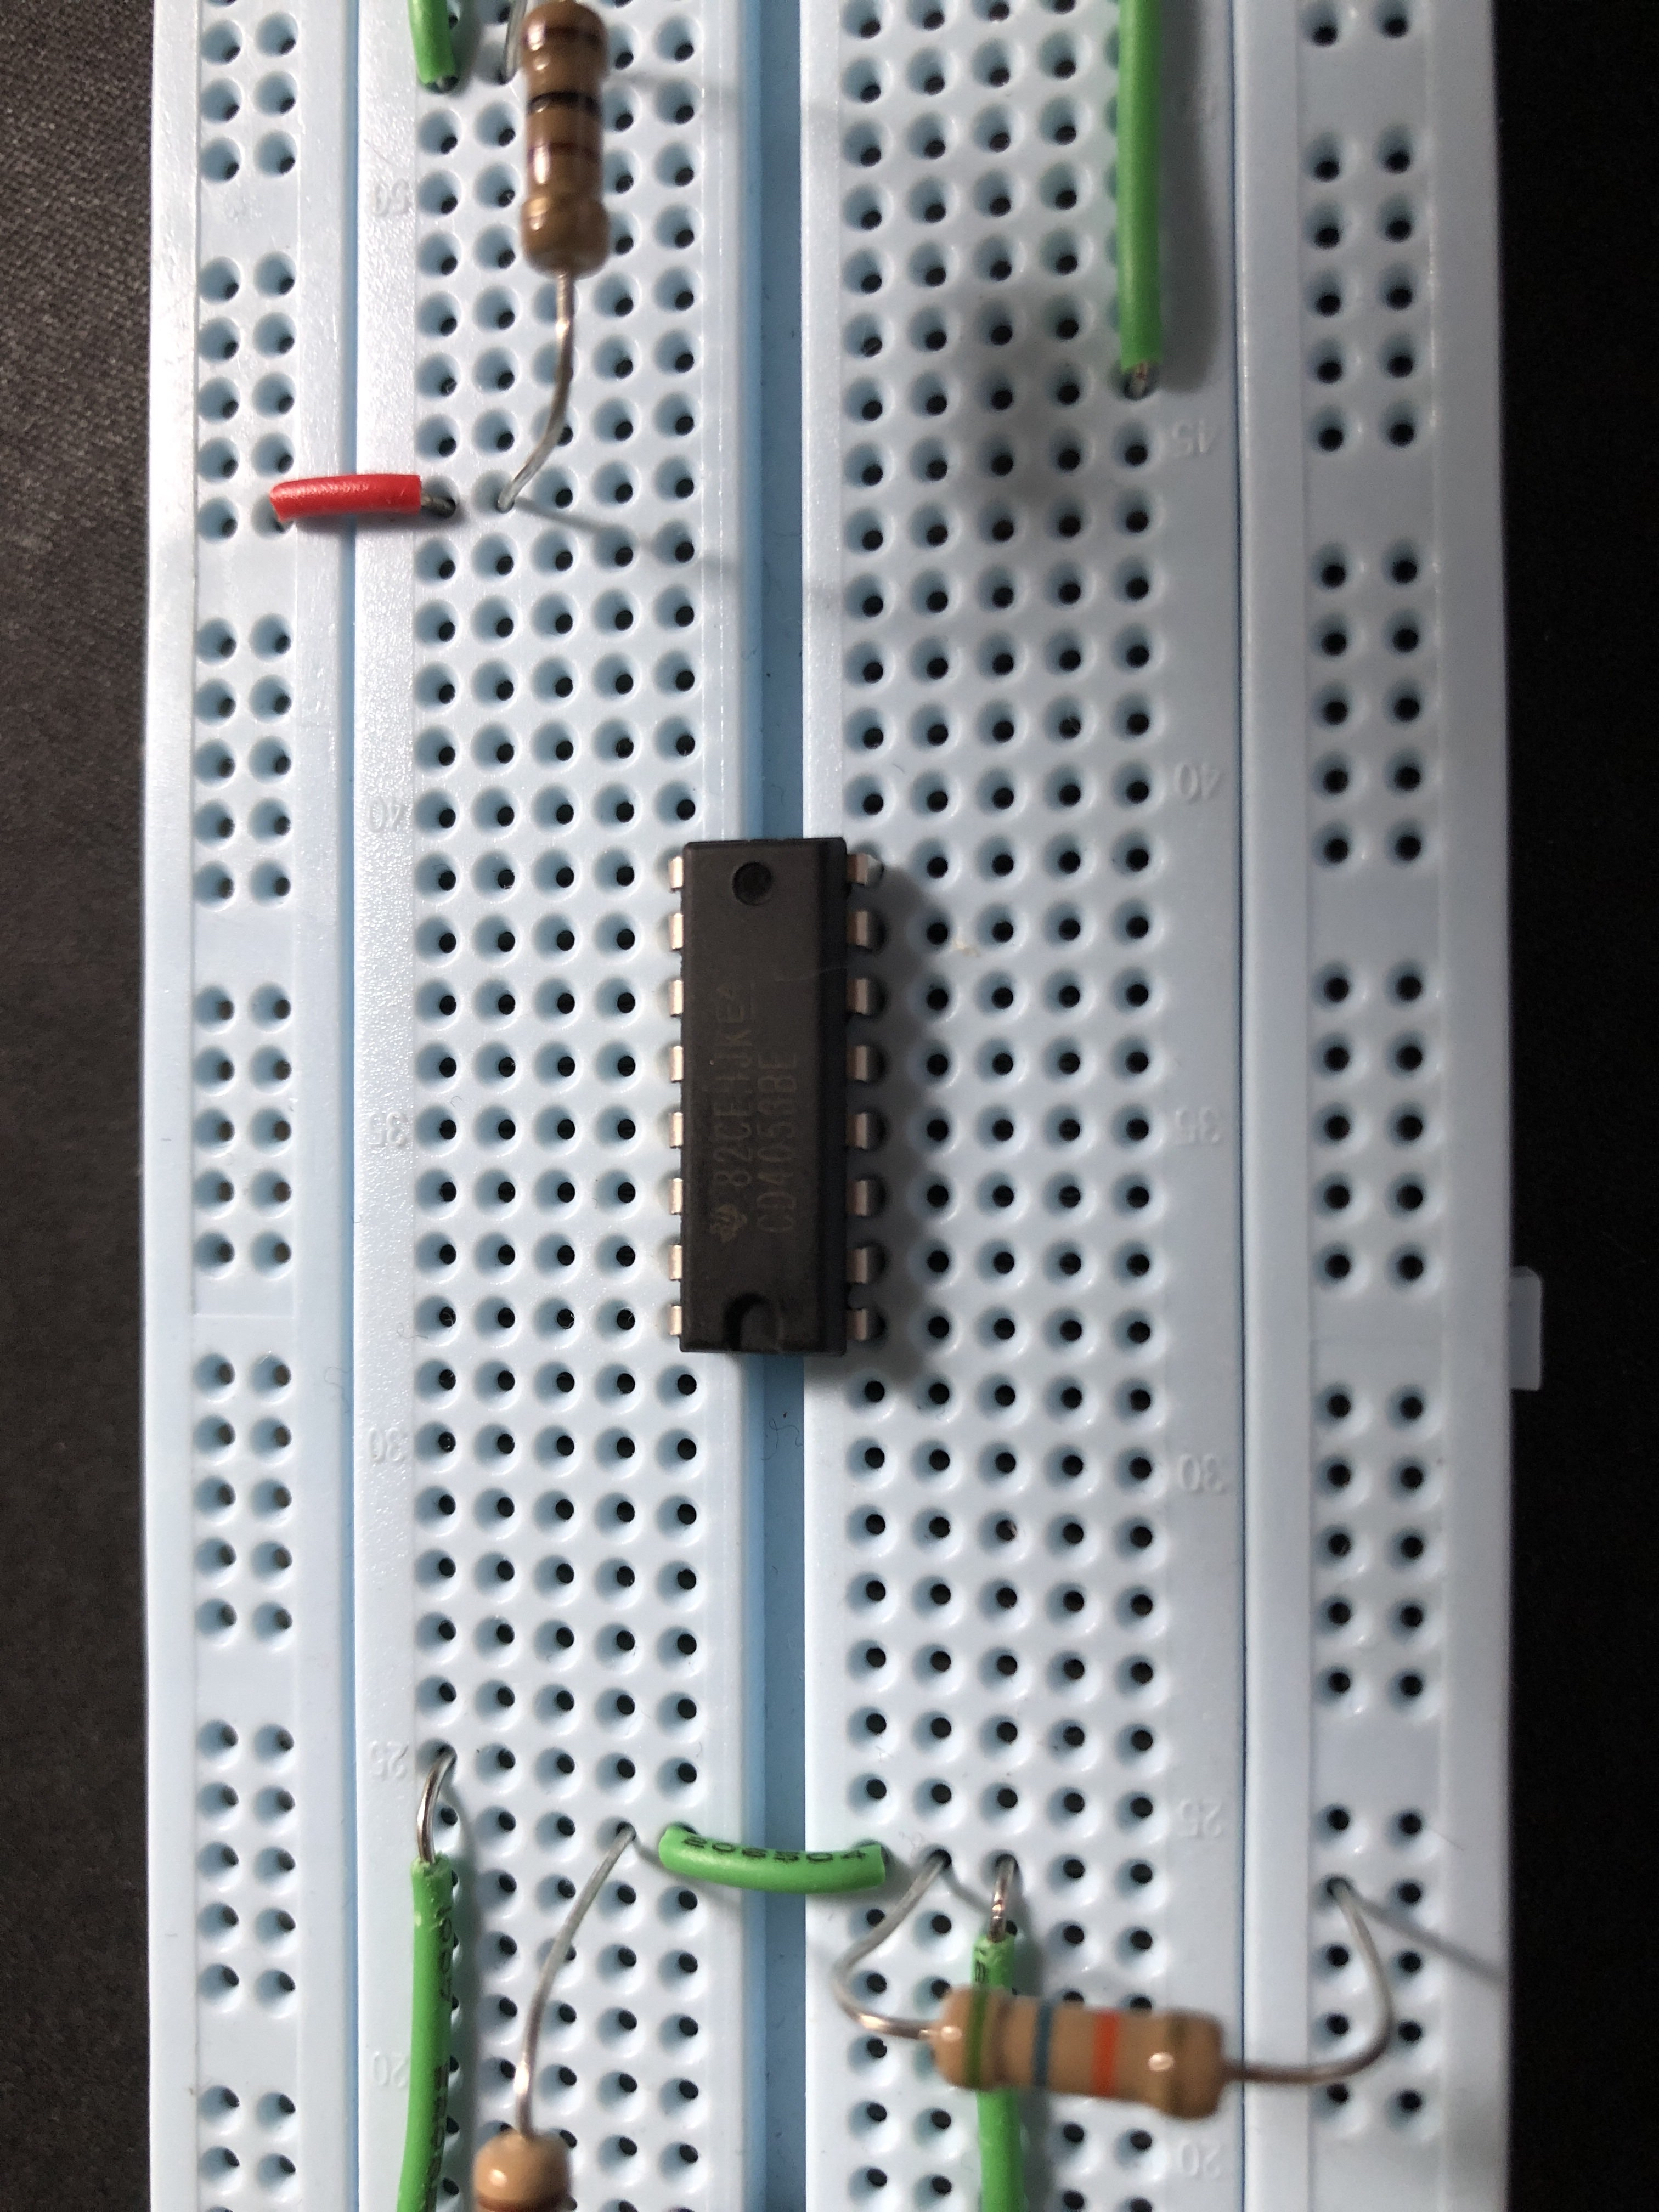
\includegraphics[width = .75\textwidth,height = .5\textwidth]{images/mux.jpg}}
\end{center}
From this we can see that the model number is \textbf{CD4053BE}. From this the datasheet can be found to be here at the following link:

\url{https://www.ti.com/general/docs/suppproductinfo.tsp?distId=10&gotoUrl=http%3A%2F%2Fwww.ti.com%2Flit%2Fgpn%2Fcd4051b}

Now we can get the pin-out from the data sheet to better understand the multiplexer:
\begin{center}
    \boxed{\includegraphics[width = .475\textwidth]{images/pinout.png}}
\end{center}
Now I can start by making the easiest connections first, $V_{DD}$ and $V_{SS}$(Ground) but first I need to find out how many volts the $V_{DD}$ on this chip is rated for. 
\begin{center}
    \boxed{\includegraphics[width = .65\textwidth]{images/maxratings.png}}
\end{center}
Now that I know I can safely tie $V_{DD}$ to 5V without damage I can give the mux $V_{SS}$ and $V_{DD}.$

The next step before I can test the operation of the mux is to use the datasheet to figure out the purpose of all of the remaining pins and to decide wether or not I need to use them.
\begin{itemize}
    \item \textbf{PIN 6:INH}
    
    INH stands for inhibit, this pin if given a logic level of one will stop the operation of the multiplexer completely, could be useful for a bonus feature for pausing or such, but for now I will tie it to ground since we want the multiplexer actually operating.
    
    Input: GND
    \item \textbf{PIN 7:$V_{EE}$}
    
    This input is the negative voltage source, according to the data sheet it seems like this is a needed input for operation of the multiplexer so I will be connecting it properly.
    
    Input: -5V
    \item \textbf{PIN OTHER:[ax, ay, bx, by, cx, cy]}
    
    These pins are the input/output pins for the multiplexers and it does work in both directions, so if needed It can decode.
    
    Input: Desired Signal
    \item \textbf{PIN 11-9:[A, B, C]}
    
    These three channels are the select bits for the multiplexer, the inputs needed to pass the correct output can be seen in the truth table below.
    
    Input: Sel Bits
\end{itemize}
\begin{center}
    \boxed{\includegraphics[width = .55\textwidth]{images/truthtable.png}}
\end{center}
After a bit of research I realized that instead of this being a 3x8 multiplexer, it is 3 1x2 multiplexers, which makes things pretty simple as I don't need to use most of those inputs to the multiplexer anyway.

After figuring out the purposed of the pins, this is the mini-circuit I ended up with.
\begin{center}
    \boxed{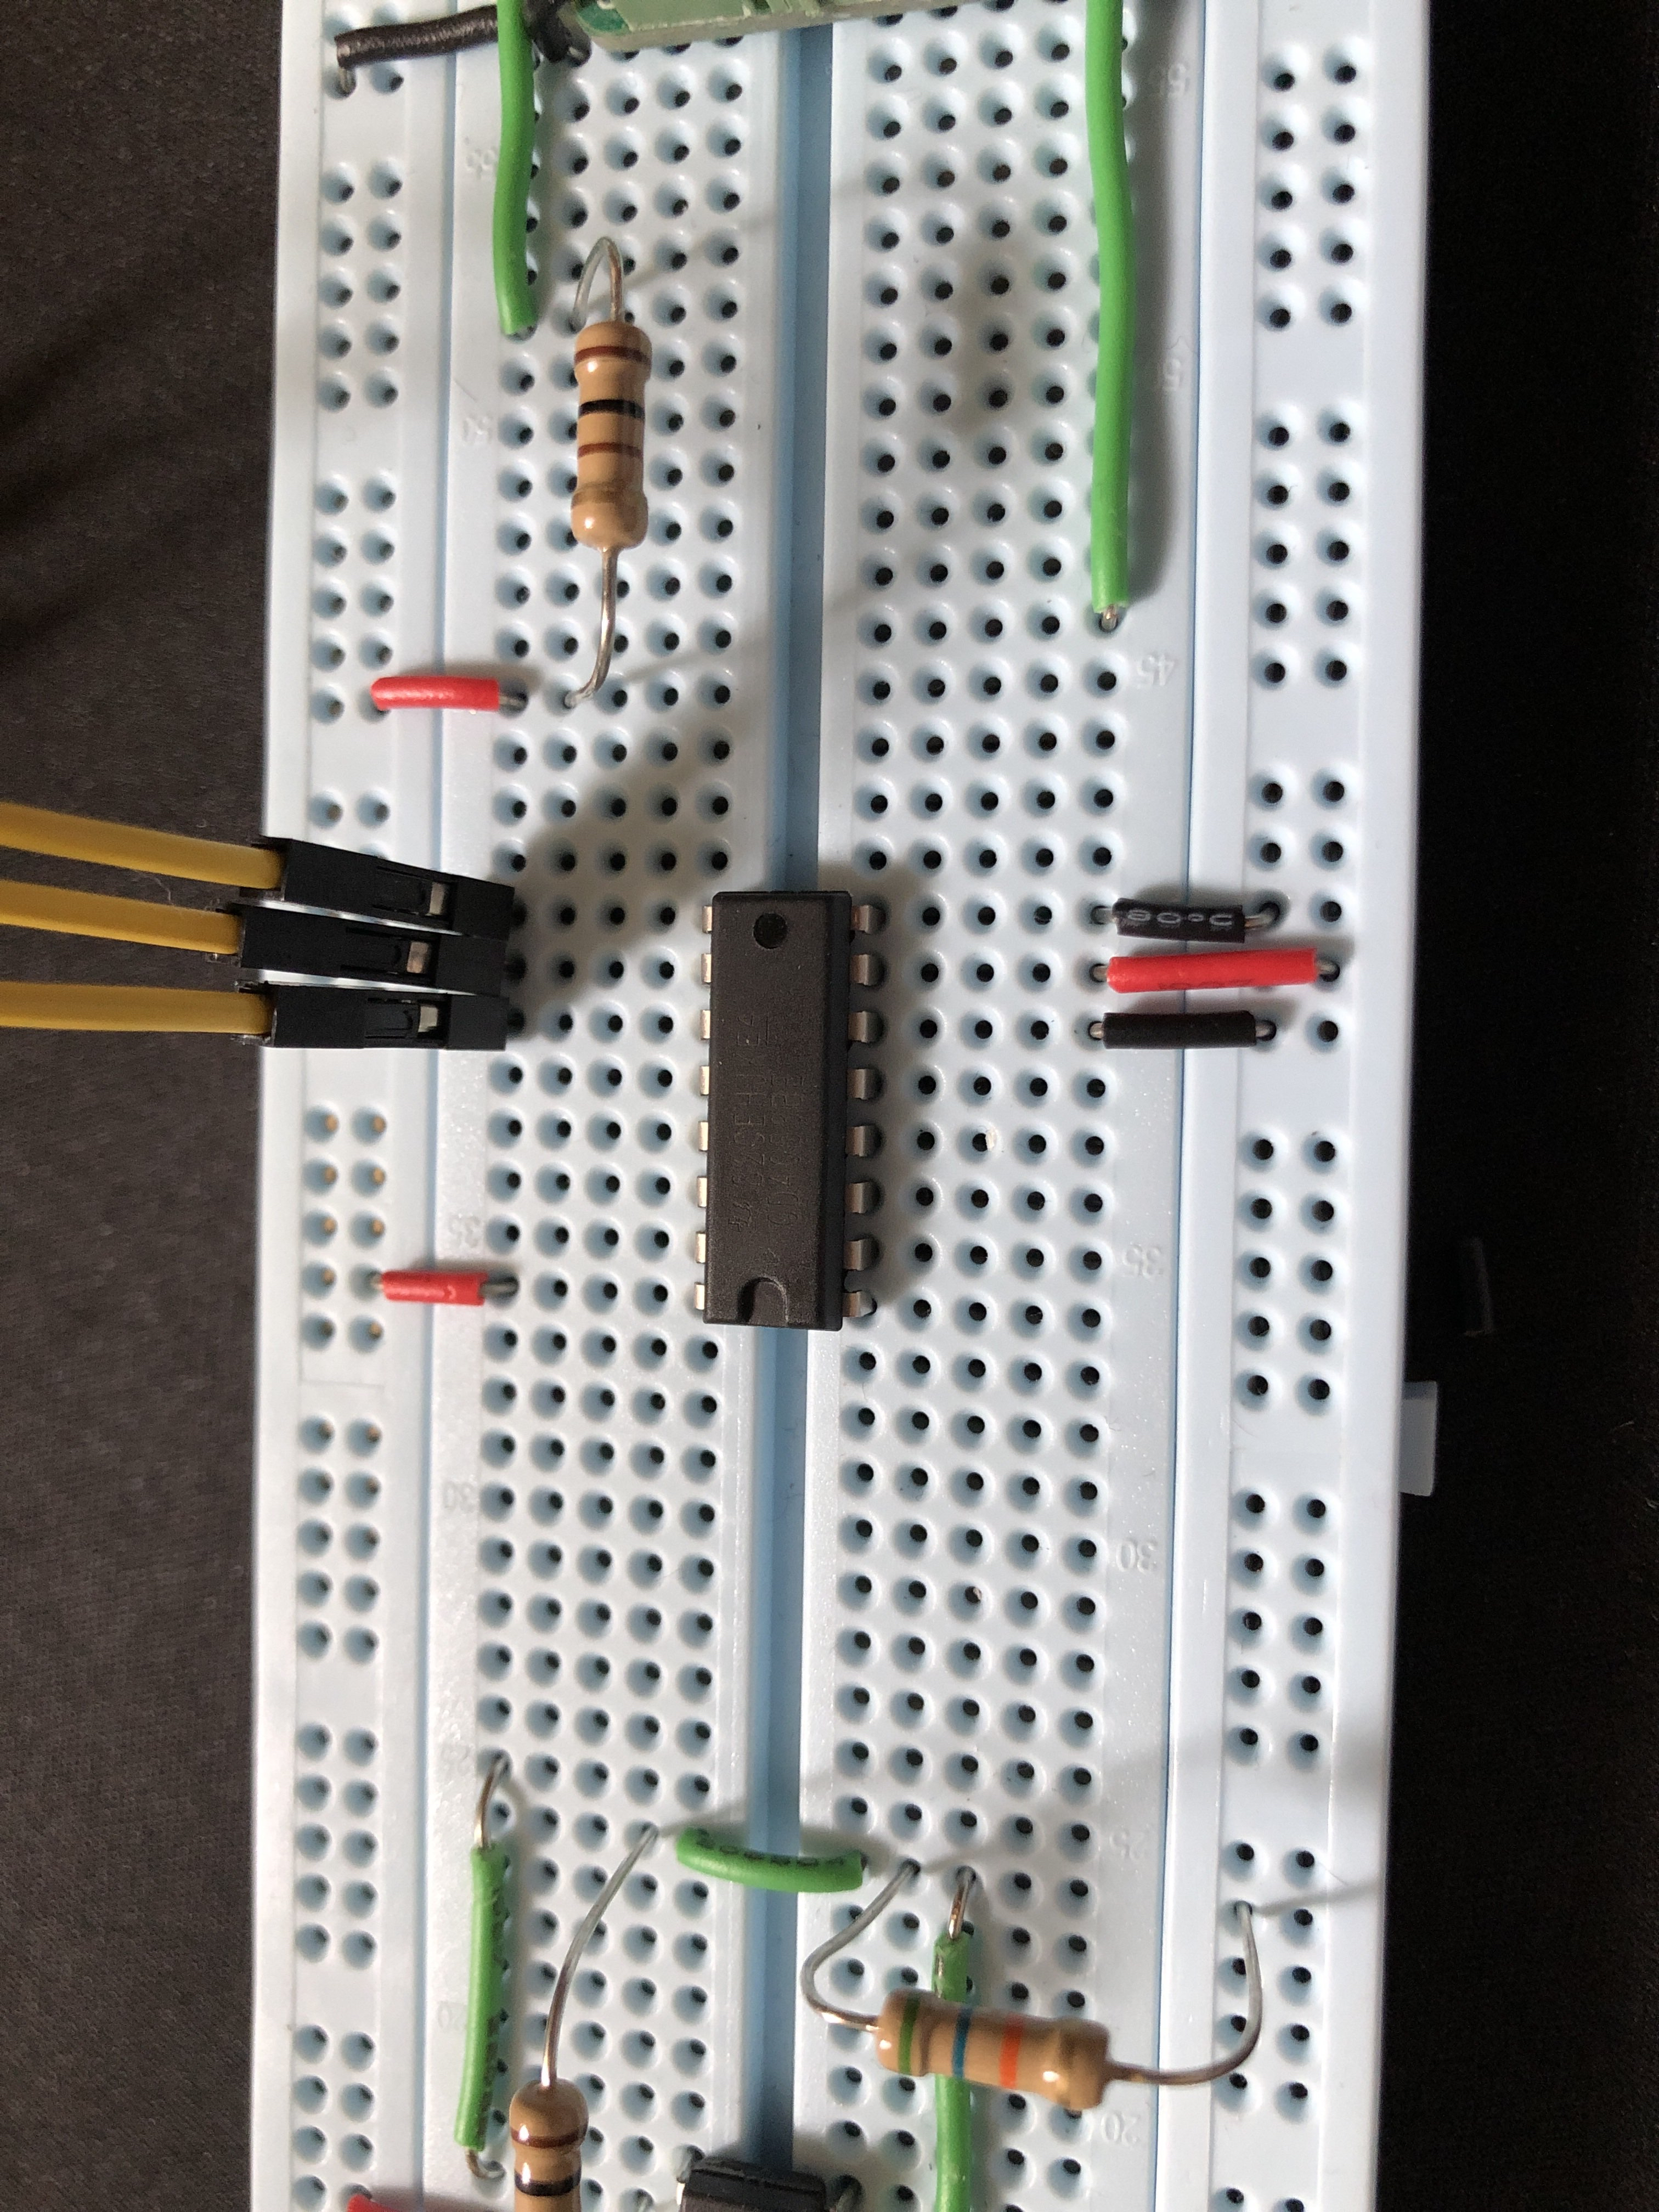
\includegraphics[width = .65\textwidth,height = .45\textwidth]{images/mux2.jpg}}
\end{center}
Now I can write some simple test code in the arduino to test out the multiplexer A.
\begin{lstlisting}[language=Arduino, caption=Multiplexer Test Code]
void setup() {
  pinMode(13, OUTPUT); // primes pin 13 for digital writing
}

void loop() {
  digitalWrite(13, HIGH); // sets the digital pin 13 on
  delay(500);            // waits for a half second
  digitalWrite(13, LOW);  // sets the digital pin 13 off
  delay(500);            // waits for a half second
}
\end{lstlisting}
Now this code will send the A select bit a high signal, then a low signal continuously which will switch the input and outputs of the multiplexer, now I need to provide the mux with proper inputs. I can do this using both channels of the wavegenerator on the AD2.
\begin{center}
    \boxed{\includegraphics[width = .85\textwidth]{images/wavegen.png}}
\end{center}
Now in theory when I turn on all components, on the oscilloscope I should see a signal that switches between noise and sin wave every half a second. If this doesn't happen I can debug and go from there.
\begin{center}
    \boxed{\includegraphics[width = .85\textwidth]{images/oscillisocpe_mux.png}}
\end{center}
Now that the multiplexer is setup when the time comes to select the proper signal input from the sensor it can be done.
\newpage
\subsubsection{Post-Filtering Amplification}
With the filtering done we need to amplify the signal even more to make it more visible and manipulable. I will be using a simple non-inverting op amp for this. Start with some simple calculations for the component values. 
\begin{center}
    \ctikzset{bipoles/length=1cm,transistors/scale=1.4,grounds/scale=1.4}
    \begin{circuitikz}[scale=1]
        \ctikzset{tripoles/mos style/arrows}
        \draw (0,0) to [vsourcesin,l=$v_i$](0,2)
        to [R,l=$R_{Si}$](1.5,2)
        to [C,l=$C_{C1}$](3,2)
        to [R,l_=$R_1$] (3,4)
        to [short,-*] (3.75,4)
        to [short, -o](3.75,4.5) node[anchor=south]{$V_{DD}$}
        (3.75,4) to [short,-] (4.5,4)
        to [R,l=$R_D$,-*] (4.5,2.75)
        to [short, -o](5.25,2.75)node[anchor=west]{$v_o$};
        \draw (3,2) to [short,*-] (3.51,2)(4.5,2) node[nmos]{};
        \draw (0,0) to [short, -*] (3,0) to [R,l_=$R_2$] (3,2) 
        (3,0) to [short, -*](4.5,0) node[ground]{} to [short] (4.5,1.22);
    \end{circuitikz}
\end{center}
There is alot of uncertainty with the transistor parameters for the transistors in our kit because they are not listed anywhere, but from experience and from ECE2214 labs I have learned that $K_n \cong 30\frac{mA}{V^2}$ and $V_{TN} \cong 1.1V$ so those are the values I will use for the transistor parameters. I want a gain so that I will be able to see the final signal but I also need to make sure I dont go under 0 volts or over 5 volts so that will be reflected in the calculations.
\begin{equation}
    5mA = 30\frac{mA}{V^2}(V_{DS}(sat))^2 \Rightarrow V_{DSt} = .408V
\end{equation}
\begin{equation}
    V_{DSQ} = \frac{V_{DD}+V_{DSt}}{2}= 2.7V
\end{equation}
\begin{center}
\end{center}
\begin{align}
    V_{DD} &=  I_{DQ}R_D + V_{DSQ}\\
    \Rightarrow 5V &=  2.5mA\cdot R_D + 2.7V\\
    \Rightarrow R_D &=  \boxed{920\Omega}
\end{align}
\begin{align}
    2.5mA &= 30\frac{mA}{V^2}(V_{GSQ}-1.1V)^2\\
     V_{GSQ} &= \pm\sqrt{\frac{2.5mA}{30\frac{mA}{V^2}}} + 1.1V\\
     V_{GSQ} &= 1.38867V
\end{align}
\begin{align}
    V_{GSQ} &= V_{DD}\left(\frac{R_2}{R_1+R_2}\right)\\
    \Rightarrow R_1\cdot V_{GSQ} &= V_{DD}(R_1||R_2)\\
    \Rightarrow R_1\cdot1.258V &= 5V\cdot100k\Omega\\
    \Rightarrow R_1 &= \boxed{360k\Omega}\\
    \Rightarrow R_2 &= \frac{V_{GSQ}R_1}{V_{DD}-V_{GSQ}}\\
    &= \boxed{138.453k\Omega}
\end{align}
\newpage
Here is the small signal equivalent for the MOSFET amplifier above.
\begin{center}
    \ctikzset{bipoles/length=1cm,transistors/scale=1.4,grounds/scale=1.4}
    \begin{circuitikz}[american currents,american voltages]
        \ctikzset{tripoles/mos style/arrows}
        \draw
        (-1.5,0) to [vsourcesin,l=$v_i$](-1.5,2)
        to [short](.5,2)
        (-1.5,0) to [short](0,0)
        (-.6,0) to [R,l_=$R_1$,*-*](-.6,2)
        (.4,0) to [R,l_=$R_2$,*-*](.4,2)
        to [short, -o](1.5,2)node[anchor=south]{G}
        to [open,v=$V_{GS}$](1.5,0)
        (0,0) to [short,-*](1.5,0)
        to [short](3,0)
        (3,0) to [short,-o](7,0)
        (3,0) node[anchor=north]{S} to [cisource,l_=$V_{GS} g_m$,invert,*-](3,2)
        to [short](5,2)
        to [short](6.5,2)
        to [short, -o](7,2)node[anchor=west]{$v_o$}
        (6,2) to [R,l=$r_o$,*-*](6,0)
        (5,2)node[anchor=south]{D} to [R, l=$R_D$,*-*](5,0);
    \end{circuitikz}
\end{center}
\begin{equation}
        A_v = -g_m(r_o||R_D) = -2\sqrt{30\frac{mA}{V^2}\cdot 2.5mA} \cdot 920\Omega = \boxed{-15.93486}
\end{equation}
\begin{center}
    So, $\boxed{R_1 = 360k\Omega}$, $\boxed{R_2 = 140k\Omega}$, and $\boxed{R_D = 920\Omega}$
\end{center}
Since this amplifier has a negative gain I also need an inverting op amp with a gain of 1 to normalize the signal after its amplified
\begin{equation}
    A_v = \frac{R_f}{R_i} \Rightarrow R_f = R_i
\end{equation}
\begin{center}
    So all I need to do to make the amplifier is pick two resistor values which are equal to each
    
    So, $\boxed{R_f = 100k\Omega}$ and $\boxed{R_i = 100k\Omega}$
\end{center}
\begin{center}
    \boxed{\includegraphics[width = .75\textwidth]{images/LTcommonsource.png}}
\end{center}
Now we can test it, but to see any meaningful information I need to graph the output in an external program such that I can give $V_{out}$ an offset off $V_{DSQ}$, I chose to do that in python. The code I used for this is below:
\begin{lstlisting}[language=Python, caption= Graphing Code]
import numpy as np
import matplotlib.pyplot as plt
from matplotlib.pyplot import figure
import pandas as pd

figure(figsize=(14, 6))

# import csv and convert to numpy array

real = pd.read_csv("C:\Users\ksbkt\OneDrive - Virginia Tech\Documents\Files\School\ECE2804\project\commonsource.csv", names=["time", "V_IN", "V_OUT"])

real.time *= 10**3
real.V_OUT *= 10**3
real.V_IN *= 10**3

# plot

plt.title("NMOS Amplifier: Physical")
plt.plot(real.time, real.V_IN, label="$V_{IN}$")
plt.plot(real.time, (real.V_OUT-4.95*10**3), label="$V_{OUT}$")
plt.xlabel("$Time(ms)$ ")
plt.ylabel("$Voltage(mV)$")
plt.legend()
plt.show()
\end{lstlisting}
\begin{center}
    \boxed{\includegraphics[width = .6\textwidth]{images/nmosampsim.png}}
\end{center}
So we clearly have a good amount of gain that will allow us to properly play around with ours signal, now I can build the circuit in real life and connect it up to the output of the filter and see what it gives me.
\begin{center}
    \boxed{\includegraphics[width = .75\textwidth]{images/nmosampreal.png}}
\end{center}
With the circuit built and hooked up we can see what the next concurrent output of the circuit will be.
\begin{center}
    \boxed{\includegraphics[width = .75\textwidth]{images/nmosampout.png}}
\end{center}
This signal is starting to look like the ones that were seen in the reference material for this project.

After this, We decided to modify the schematic for the amplifier a bit and that can be seen detailed in calvins section.
\newpage
\subsubsection{Finding DC Value of Signal}

Since we already know where the systolic and diastolic peaks are from calculating the heart rate all that needs to be done to calculate the DC level (or average) of the signal, that will give us all the needed information to calculate the R ratio when the time comes.

This can be done entirely digitally using a running average of the incoming AC signal like so:
\begin{lstlisting}[language=Arduino, caption= DC Average Code]
// readings to keep track of, the more readings the more smooth but less reactive to change
const int numReadings = 25;    

int readings[numReadings];      // the readings from the analog input
int readIndex = 0;              // the index of the current reading
int total = 0;                  // the running total
int average = 0;                // the average

int inputPin = A0;

void setup() {
  Serial.begin(9600);
  // initialize all the readings to 0
  for (int i = 0; i < numReadings; i++) {
    readings[i] = 0;
  }
}

void loop() {
  total = total - readings[readIndex];
  readings[readIndex] = analogRead(inputPin);
  total = total + readings[readIndex];
  readIndex = readIndex + 1;

  if (readIndex >= numReadings) {
    readIndex = 0;
  }

  average = total / numReadings;
  Serial.println(average);
  delay(1);        // delay in between reads for stability
}
\end{lstlisting}
But the only problem with this strategy of finding the DC level is that since the input signal is not a perfect sinusoid, taking the average will not cancel out the AC component of the signal, to avoid this another method we can use is to take the center point of the tallest peak and the lowest valley which will give us the DC level, according to the following formula:
\begin{equation}
    V_{DC} = \frac{V_{peak}+V_{valley}}{2}
\end{equation}
Now all we need for this is to sample the data at the proper peak and valley of the signal and make the calculations digitally.
\begin{center}
    \boxed{\includegraphics[width = .4\textwidth]{images/DC_estimation.png}}
\end{center}
Above is a graphical representation of what will be done in the other version of the code.
\newpage
\subsubsection{Clamping Circuit}
After the complete signal is achieved, it is slightly under where we want it to be so I need to design a clamping circuit to bring it back to a positive voltage such that we can input it into the arduino ADC without damaging the pins.

The signal currently rests at about -2.1V, So I will clamp it 2.5V in upwards. I pick the biggest capacitor in the kit for the circuit.
\begin{center}
    \boxed{\includegraphics[width = .7\textwidth]{images/LTClamp.png}}
\end{center}
This is an ideal diode so the voltage is set to 2.5V to get the clamp but in real life it would be 1.8V from a voltage divider because of the .7V forward voltage drop. The LTSpice simulation plot is below:
\begin{center}
    \boxed{\includegraphics[width = .7\textwidth]{images/LTclamp_plot.png}}
\end{center}
The capacitor charging took up some of the wave but that would only happen on the start up.

Next I can build the circuit in real life, replacing the voltage source with a voltage divider.
\begin{center}
    \boxed{\includegraphics[width = .875\textwidth, height = .575\textwidth]{images/clamper.jpg}}
\end{center}
From that I can get a simulation to see if it is clamping properly, I will use the AD2 wave  gen to create a test signal for me for this.
\begin{center}
    \boxed{\includegraphics[width = .8\textwidth]{images/clamperplot.png}}
\end{center}
This will allow for the signal to be inputted into the arduino without damaging the pins
\newpage
\subsubsection{Displaying Waveform}
One of the objectives of this project is to display the sensor output after it has been processed on to the LCD screen, my code for this and an example picture of what it looks like is below.
\begin{lstlisting}[language=Arduino, caption= Waveform Display Code]
#include <Wire.h>
#include <SPI.h>
#include <Adafruit_GFX.h>
#include <Adafruit_SSD1306.h> 

//creating display object
#define SCREEN_WIDTH 128 // OLED display width
#define SCREEN_HEIGHT 32 // OLED display height
Adafruit_SSD1306 display(SCREEN_WIDTH, SCREEN_HEIGHT, &Wire, -1);

//variable declarations
const int ANALOG_INPUT_PIN = A0;
const int MIN_ANALOG_INPUT = 0;
const int MAX_ANALOG_INPUT = 1023;
const int LOOP_DELAY = 5; // change to slow down how often to read and graph value

int circularBuffer[SCREEN_WIDTH]; 
int writeIndex = 0; // tracks where we are in the circular buffer

int graphHeight = SCREEN_HEIGHT - 10;

void setup() {
  Serial.begin(9600);
  //check if display is properly conectted, if not stop program
  if (!display.begin(SSD1306_SWITCHCAPVCC, 0x3C)) { // Address 0x3D for 128x64
    Serial.println(F("SSD1306 allocation failed"));
    for (;;); // Don't proceed, loop forever
  }
  //initalize display
  display.clearDisplay();
  display.setTextSize(1);
  display.setTextColor(WHITE, BLACK);
  display.setCursor(0, 0);
  display.display();
  delay(500);
  display.clearDisplay();
}

void loop() {
  //read inputs
  int analogVal = analogRead(ANALOG_INPUT_PIN);
  circularBuffer[writeIndex++] = analogVal;
      
  if(writeIndex >= display.width()){
    writeIndex = 0;
  }

  //display heartrate above graph
  display.clearDisplay();
  display.setCursor(0, 0);
  int16_t  x1, y1;
  uint16_t w, h;
  display.getTextBounds("XX bpm", 0, 0, &x1, &y1, &w, &h);
  display.setCursor(display.width() - w, 0);
  display.print(bpm);
  display.print(" bpm");

  //for loops to draw the graph itself
  int xPos = 0; 
  for (int i = writeIndex; i < display.width(); i++){
    int analogVal = circularBuffer[i];
    drawLine(xPos, analogVal);
    xPos++;
  }
  for(int i = 0; i < writeIndex; i++){
    int analogVal = circularBuffer[i];
    drawLine(xPos, analogVal);
    xPos++;;
  }
  
  display.display();
  //Slight delay to not sample too often
  delay(LOOP_DELAY);
}

//helper function to draw individuial lines that make up the graph
void drawLine(int xPos, int analogVal){
  int lineHeight = map(analogVal, MIN_ANALOG_INPUT, MAX_ANALOG_INPUT, 0, graphHeight);
  int yPos = display.height() - lineHeight;
  display.drawFastVLine(xPos, yPos, lineHeight, SSD1306_WHITE);
}
\end{lstlisting}
\begin{center}
    \boxed{\includegraphics[width = .8\textwidth]{images/display_waveform.png}}
\end{center}
This gives a good indication to the user if they are seating their finger properly on the sensor or not, and can not only see that heart rate in bpm but see that actual graph that the number is derived from.
\newpage
\subsubsection{Calculating Heartrate}
Now we will use a algorithm of sorts to detect peaks. It involved storing the data inputs, and based on their magnitudes relative to each other the code decides if there is a peak or not, and by storing the time that the last two beats occured and plugging it into the a formula that calculates the amount of beats per minute based on those three beat timings.

Only portions of code relevant to heartrate calculation are shown here.
\begin{lstlisting}[language=Arduino, caption= Heartrate Code]
#include <Wire.h>
#include <SPI.h>
#include <Adafruit_GFX.h>
#include <Adafruit_SSD1306.h> 

//creating display object
#define SCREEN_WIDTH 128 // OLED display width
#define SCREEN_HEIGHT 32 // OLED display height
Adafruit_SSD1306 display(SCREEN_WIDTH, SCREEN_HEIGHT, &Wire, -1);

//variable declarations
#define sampleSize 4
#define riseThreshold 5

const int ANALOG_INPUT_PIN = A0;
const int LOOP_DELAY = 5;

float bpmVals[sampleSize], sum;
long int now, ptr;
float last, bpmIn, start;
float first, second, third, before;
bool peak;
int beat_count, i, bpm;
long int last_beat;

void setup() {
  Serial.begin(9600);
  //initialize variables
  for (int i = 0; i < sampleSize; i++)
    bpmVals[i] = 0;
  sum = 0;
  ptr = 0;
}

void loop() {
  //read inputs
  int analogVal = analogRead(ANALOG_INPUT_PIN);
  Serial.println(analogVal);
  circularBuffer[printptr++] = analogVal;
  //print heart rate
  display.clearDisplay();
  display.setCursor(0, 0);
  int16_t  x1, y1;
  uint16_t w, h;
  display.getTextBounds("XXX bpm", 0, 0, &x1, &y1, &w, &h);
  display.setCursor(display.width() - w, 0);
  display.print(bpm);
  display.print(" bpm");
  
  
  
  
  
  i = 0;            //counter variable
  start = millis(); //recording current time to variable called start
  bpmIn = 0.0;      //setting input variable to zero
  // gets initial data
  do{
    bpmIn += analogRead (ANALOG_INPUT_PIN);
    i++;
    now = millis();
  }while (now < start + 20);  
  //computes rolling average to smooth any ADC flaws
  bpmIn /= i;  
  sum -= bpmVals[ptr];
  sum += bpmIn;
  bpmVals[ptr] = bpmIn;
  last = sum / sampleSize;
  // "alorithm" used to detect heart beats
  if (last > before){
    beat_count++;
      if (!peak && beat_count > riseThreshold){
      peak = true;
      first = millis() - last_beat;
      last_beat = millis();
      bpm = 60000.0 / (0.4 * first + 0.3 * second + 0.3 * third);
      if(bpm < 10)
        bpm = 0;
      third = second;
      second = first;
      }
  }else{
    peak = false;
    beat_count = 0;
  }
  //end of loop "maintainence"
  before = last;
  ptr++;
  ptr %= sampleSize;
  display.display();
  delay(LOOP_DELAY);
}

// helper function to draw graph
void drawLine(int xPos, int analogVal){
  int lineHeight = map(analogVal, MIN_ANALOG_INPUT, MAX_ANALOG_INPUT, 0, graphHeight);
  int yPos = display.height() - lineHeight;
  display.drawFastVLine(xPos, yPos, lineHeight, SSD1306_WHITE);
}
\end{lstlisting}
Now we have working heartrate calculation. The image of what that looks like on the display was shown in the previous section. Now the only calculations left to do is the calculations for the R ratio which will give us all project specifications needed. But to calculate R ratio I need a way to switch the ired and red led on and off, since I dont have anymore MOSFETS to spare I need to figure out a different way to do it.
\newpage
\subsubsection{Calculating SpO2 (W.I.P)}
Here is the partial code for calculating SpO2, it is complete except for I need to hookup the ired signal input, but all the code for calculating the R values is in place other than that.
\begin{lstlisting}[language=Arduino, caption= SpO2 Calculation Code]
#include <Wire.h>
#include <SPI.h>
#include <Adafruit_GFX.h>
#include <Adafruit_SSD1306.h> 

//creating display object
#define SCREEN_WIDTH 128 // OLED display width
#define SCREEN_HEIGHT 32 // OLED display height
Adafruit_SSD1306 display(SCREEN_WIDTH, SCREEN_HEIGHT, &Wire, -1);

//variable declarations
#define sampleSize 4
#define riseThreshold 5

const int ANALOG_INPUT_PIN = A0;
const int MIN_ANALOG_INPUT = 0;
const int MAX_ANALOG_INPUT = 1023;
const int LOOP_DELAY = 5;

int circularBuffer[SCREEN_WIDTH]; 
int printptr = 0; 

int graphHeight = SCREEN_HEIGHT - 10;

float bpmVals[sampleSize],
      peaks[5],
      valleys[5],
      min_val,
      max_val,
      peakSum,
      valleySum,
      sum,
      last,
      bpmIn,
      start,
      first,
      second,
      third,
      before;
long int now,
         ptr,
         peakptr,
         valleyptr;
bool peak;
int beat_count, i, bpm;
long int last_beat;

void setup() {
  Serial.begin(9600);
  //check if display is properly conectted, if not stop program
  if (!display.begin(SSD1306_SWITCHCAPVCC, 0x3C)) { // Address 0x3D for 128x64
    Serial.println(F("SSD1306 allocation failed"));
    for (;;); // Don't proceed, loop forever
  }
  //initalize display
  display.clearDisplay();
  display.setTextSize(1);
  display.setTextColor(WHITE, BLACK);
  display.setCursor(0, 0);
  display.display();
  delay(500);
  display.clearDisplay();
  //initialize variables
  for (int i = 0; i < sampleSize; i++)
    bpmVals[i] = 0;
  sum = 0;
  ptr = 0;
  peakptr = 0;
  valleyptr = 0;
}

void loop() {
  //read inputs
  int analogVal = analogRead(ANALOG_INPUT_PIN);
  Serial.println(analogVal);
  if(analogVal < min_val){
    min_val = analogVal;
  }
  if(analogVal > max_val){
    max_val = analogVal;
  }
  circularBuffer[printptr++] = analogVal;
  //print heart rate
  display.clearDisplay();
  display.setCursor(0, 0);
  int16_t  x1, y1;
  uint16_t w, h;
  display.getTextBounds("XXX bpm", 0, 0, &x1, &y1, &w, &h);
  display.setCursor(display.width() - w, 0);
  display.print(bpm);
  display.print(" bpm");

  //resets waveprint pointer if needed
  if(printptr >= display.width()){
    printptr = 0;
  }
  
  //for loops to draw the graph itself
  int xPos = 0; 
  for (int i = printptr; i < display.width(); i++){
    int analogVal = circularBuffer[i];
    drawLine(xPos, analogVal);
    xPos++;
  }
  for(int i = 0; i < printptr; i++){
    int analogVal = circularBuffer[i];
    drawLine(xPos, analogVal);
    xPos++;;
  }
  
  i = 0;            //counter variable
  start = millis(); //recording current time to variable called start
  bpmIn = 0.0;      //setting input variable to zero
  // gets initial data
  do{
    bpmIn += analogRead (ANALOG_INPUT_PIN);
    i++;
    now = millis();
  }while (now < start + 20);  
  //computes rolling average to smooth any ADC flaws
  bpmIn /= i;  
  sum -= bpmVals[ptr];
  sum += bpmIn;
  bpmVals[ptr] = bpmIn;
  last = sum / sampleSize;
  // "algorithm" used to detect heart beats
  if (last > before){
    beat_count++;
      if (!peak && beat_count > riseThreshold){
      peak = true;
      first = millis() - last_beat;
      last_beat = millis();
      bpm = 60000.0 / (0.4 * first + 0.3 * second + 0.3 * third);
      
      peakSum -= peaks[peakptr];
      peakSum += max_val;
      peaks[peakptr] = max_val;
      peakptr++;
      max_val = 0;

      valleySum -= valleys[valleyptr];
      valleySum += min_val;
      valleys[valleyptr] = min_val;
      valleyptr++;
      min_val = 1024;
      
      Serial.print("peak:"); Serial.print(peakSum/5); Serial.print(" ");
      Serial.print("valley:"); Serial.print(valleySum/5); Serial.print(" ");

      float peakAvg = peakSum/5;
      float valleyAvg = valleySum/5;
 
      float ACred = peakAvg-valleyAvg;
      //float ACired =;                         code chunks requiring ired
      float DCred =(peakAvg+valleyAvg)/2;
      //float DCired = ;                        code chunks requiring ired
      
      //R = (()/())/(()/());                    code chunks requiring ired

      if(bpm < 10)
        bpm = 0;
      third = second;
      second = first;
      }
  }else{
    peak = false;
    beat_count = 0;
  }
  //end of loop "maintainence"
  before = last;
  ptr++;
  peakptr %= 5;
  valleyptr %= 5;
  ptr %= sampleSize;
  display.display();
  delay(LOOP_DELAY);
}
\end{lstlisting}
\newpage
\subsubsection{Assembly}
The first thing I did to begin assembly of the circuit was to build the trans-conductance op amp, and the filters, this way by the time I get out of those two sections I have a clean signal, which only needs to be amplified, and can then begin to be prepped for calculations.
\begin{center}
    \boxed{\includegraphics[width = .875\textwidth, height = .575\textwidth]{images/kavin_assembly_1.jpg}}
\end{center}
After this, I cleaned up the filters a bit making them slightly more compact so that I would have more space to work with, then I made the common source amplifier, which included an inverting op amp with a gain of one, and finally a clamping circuit to bring the signal back to the positive voltage range such that it can be processed by the arduinio since it will break if given too negative of a voltage.
\begin{center}
    \boxed{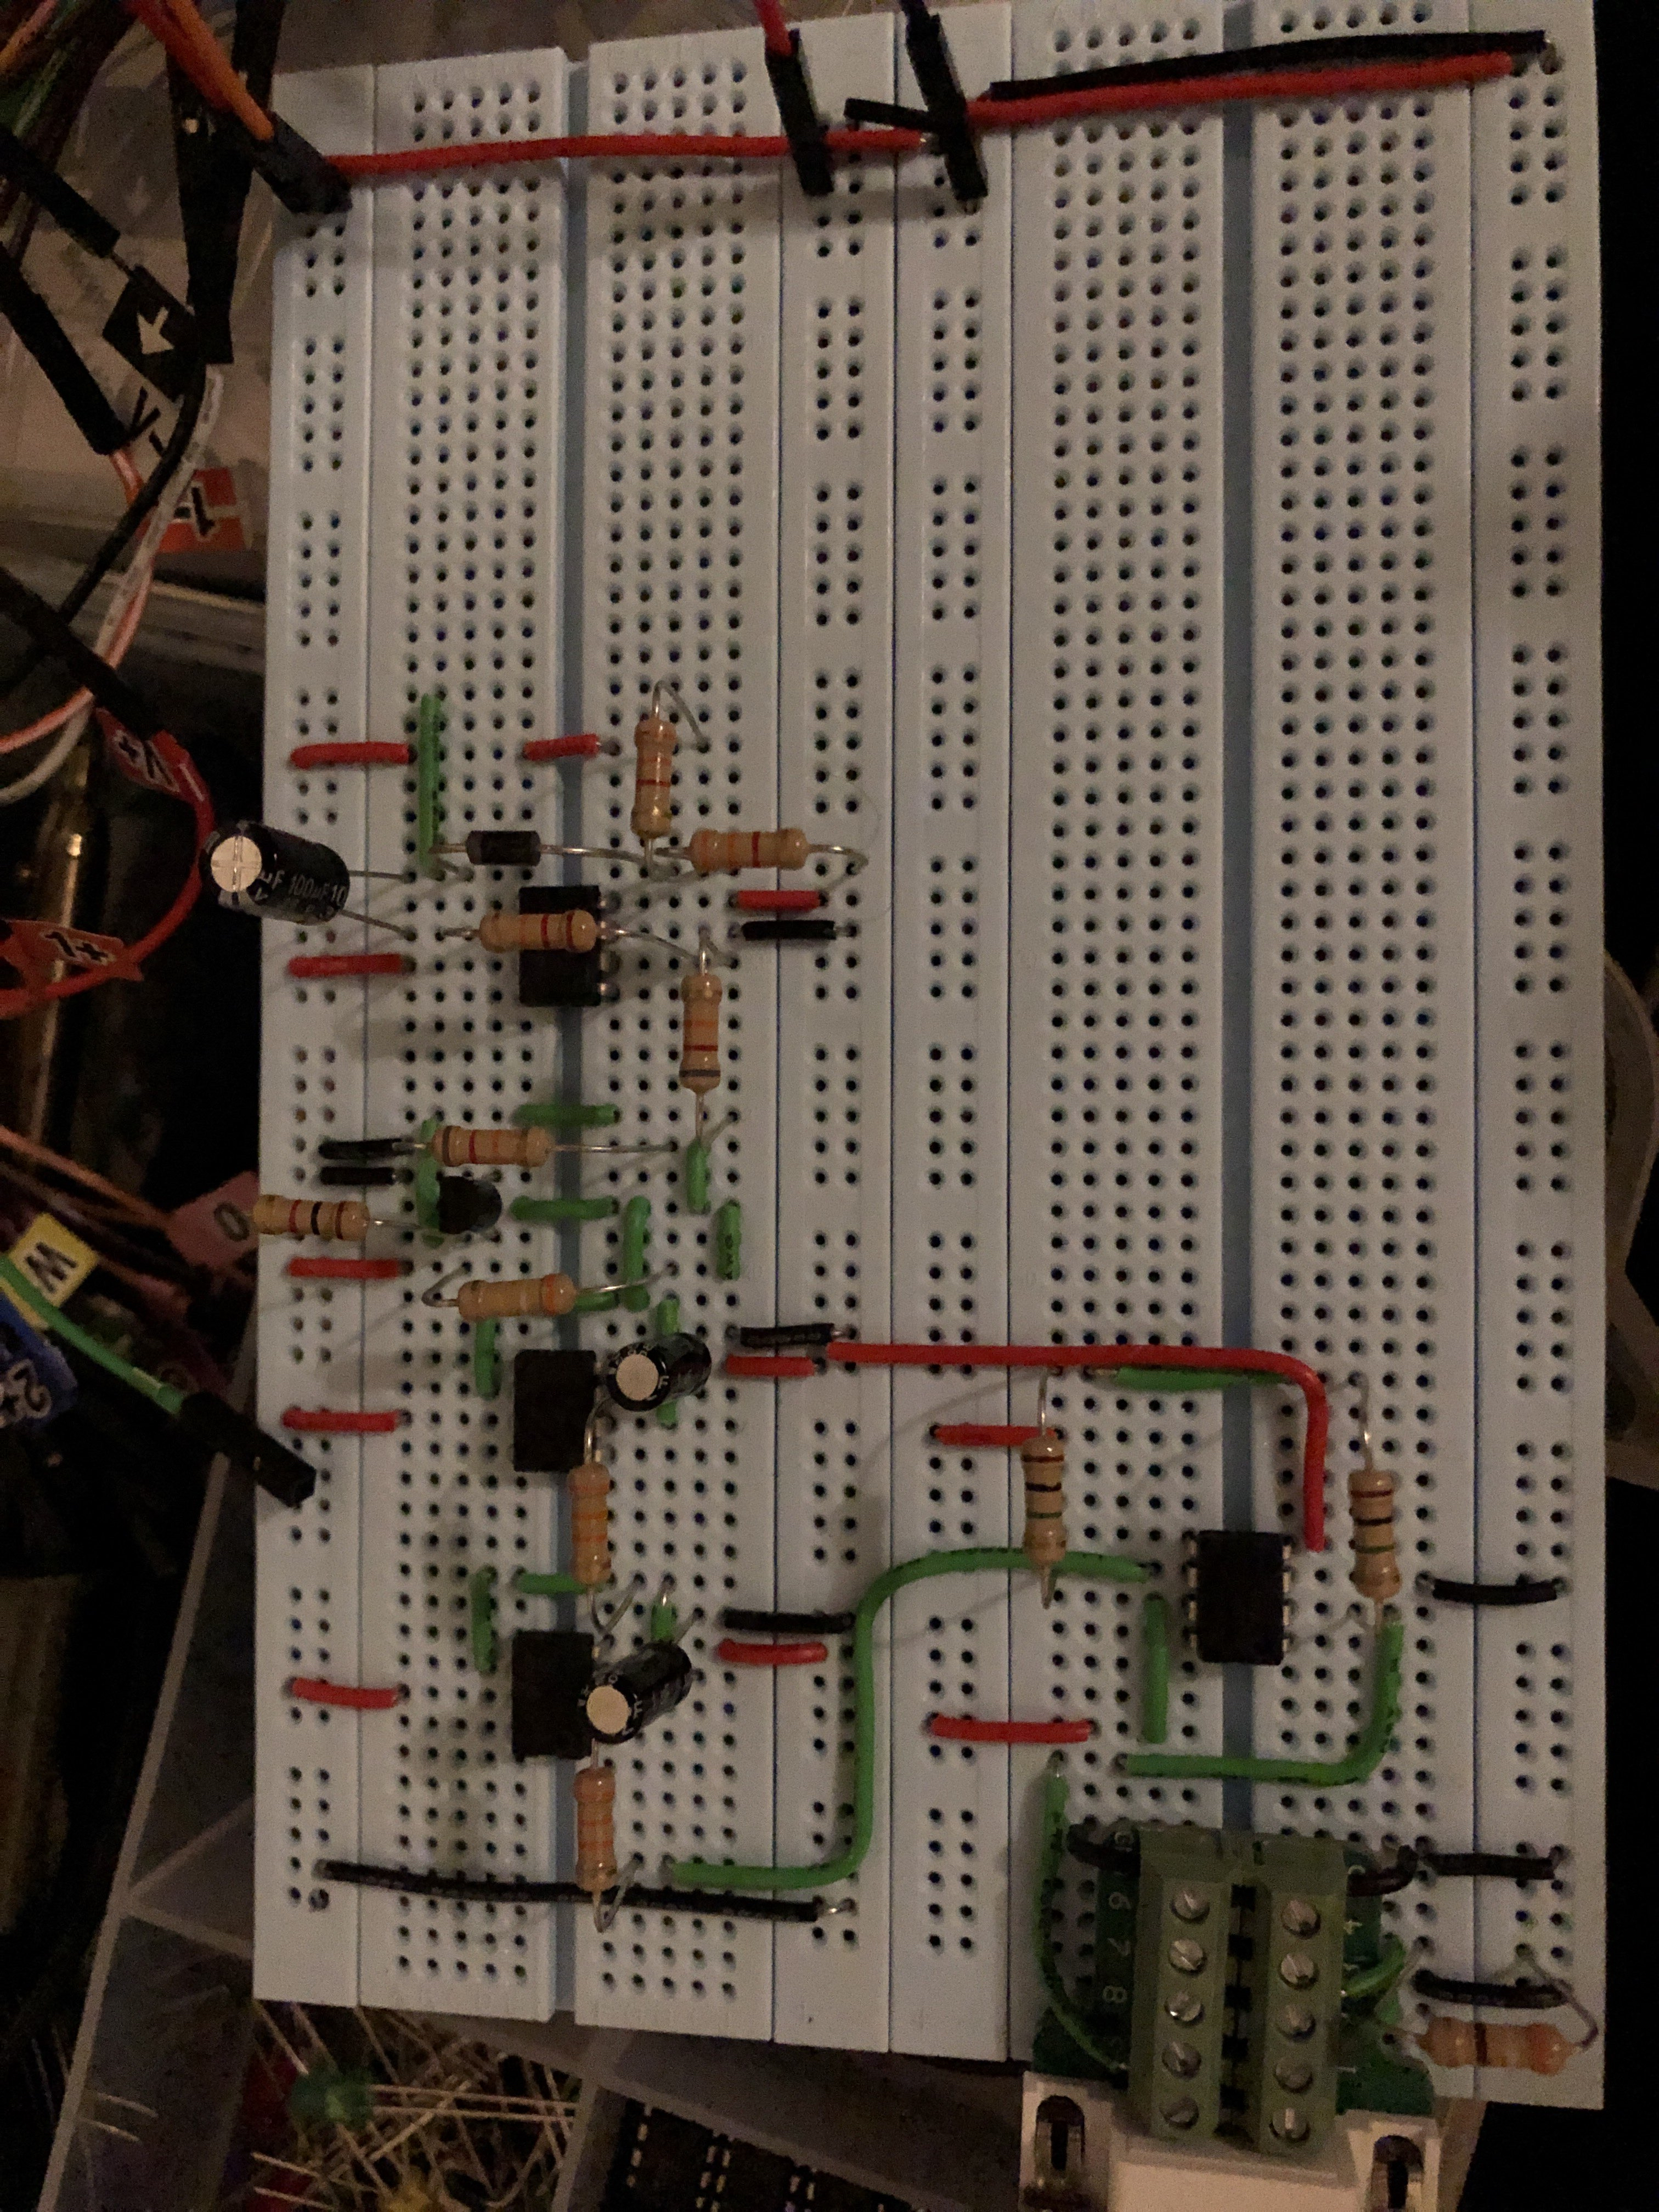
\includegraphics[width = .875\textwidth, height = .575\textwidth]{images/kavin_assembly_2.jpg}}
\end{center}
The next thing I did to assemble the circuit was to take the output of the previous sections, funnel it into the arduino and hooked the arduino up to the display
\begin{center}
    \boxed{\includegraphics[width = .875\textwidth, height = .575\textwidth]{images/kavin_complete_circuit.jpg}}
\end{center}
after that I rearranged some things and added in the multiplexer to choose between the two signals, red and ired. This will allow me to give the arduino enough information to calculate SPo2
\begin{center}
    \boxed{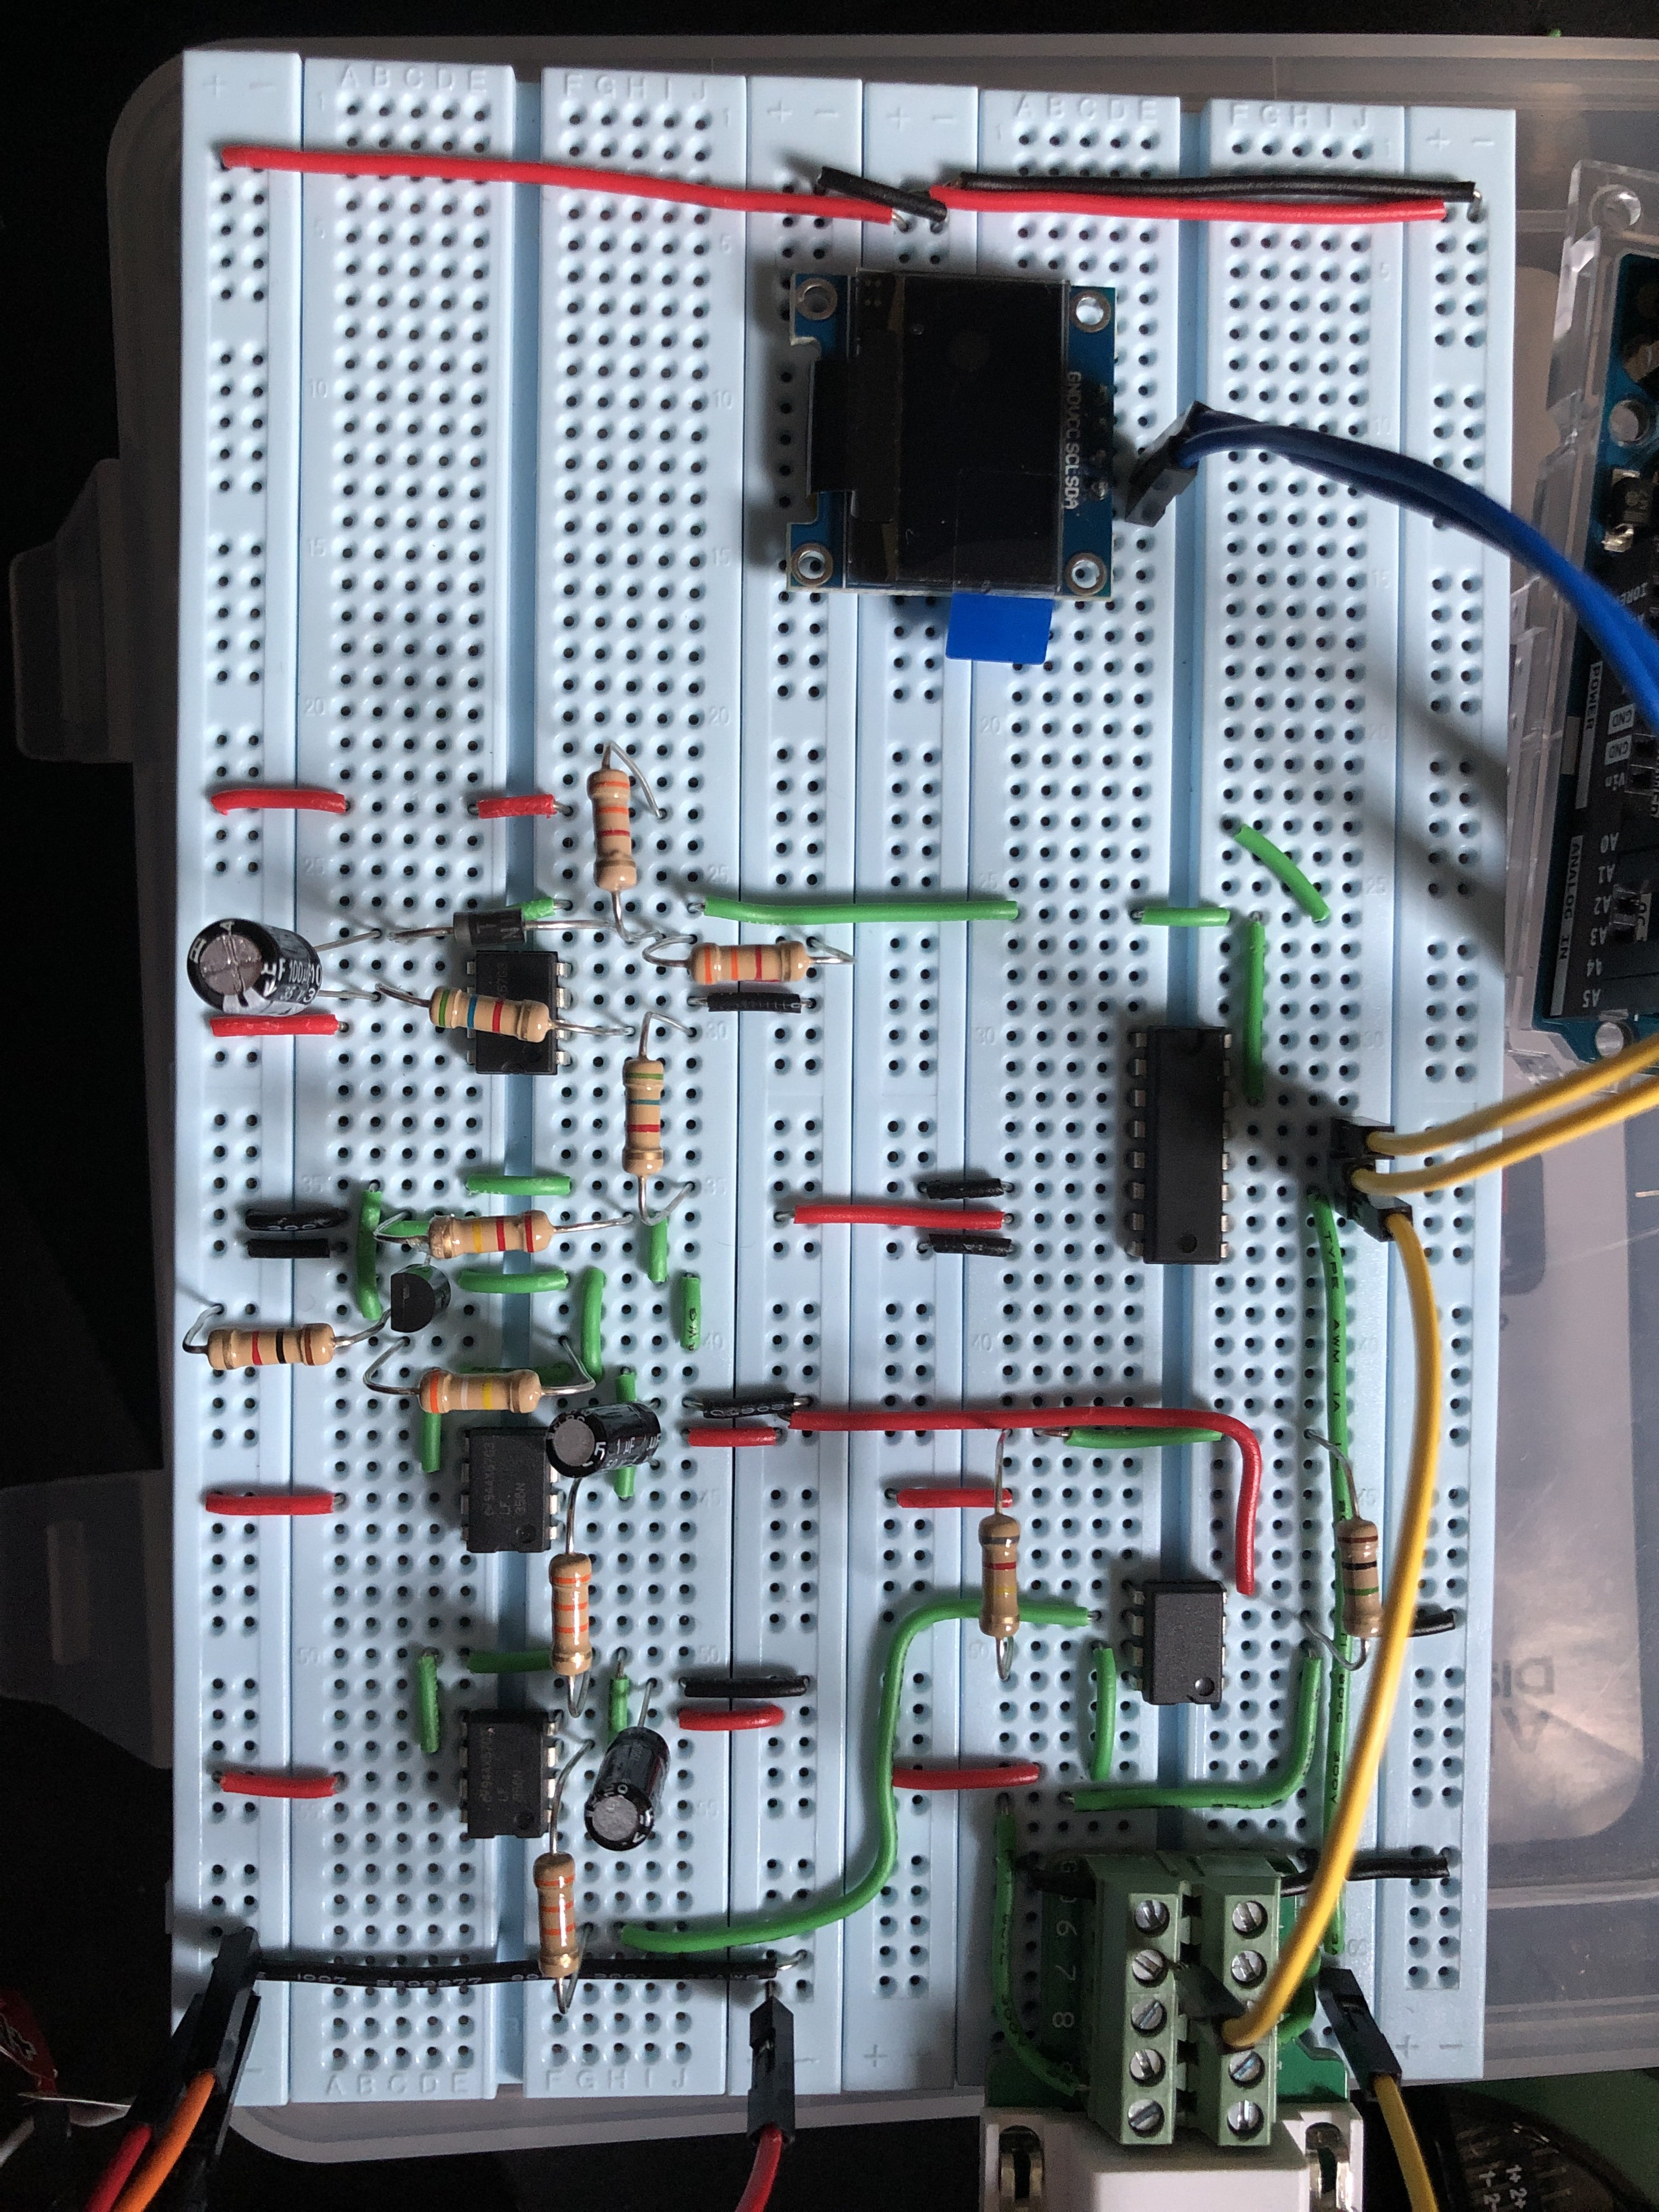
\includegraphics[width = .875\textwidth, height = .575\textwidth]{images/kavin_complete_circuit2.jpg}}
\end{center}
From here most of the circuitry is complete, some changes could be made in certain places to make the signal more consistent and easier to read, but since that is independent of rest of the programming and other changes, it can happen at any time.
\newpage
\section{Conclusion}
\subsection{Calvin}
This week I believe there has been a lot done with a readable signal along with the heart rate being calculated. The following weeks are going to be used to improve the circuit for additional stability, which will involve making adjustments to the common source amplifier due to it being determined to be the cause of the instability of the circuit. I will also be helping Kavin with the final calculations of the SpO2 value along with helping combine the code from both ends together.
\subsection{Kavin}
This week I think  we got alot done, next week my focus is on making my code more clean and readable, as well as finishing the multiplexer part of the circuit to be able to intake the ired signal needed for calculating SpO2. Another important consideration is to make the sensor easier to "get in the groove" of, as it is it takes a bit of fiddling to make the signal show up properly, so I need to figure out a way to make it more stable.
\newpage
\section{Sources}
    [1]S.-S. Oak and P. Aroul “How to Design Peripheral Oxygen Saturation (SpO2) and Optical Heart Rate Monitoring (OHRM) Systems Using the AFE4403 2015” Texas Instruments Inc., Dallas, Texas, SLAA655, 2015, Accessed on Feb. 15, 2021. [Online] Available: https://www.ti.com/lit/an/slaa655/slaa655.pdf.
    
    [2]S. Lopez “Pulse Oximeter Fundamentals and Design” Freescale Semiconductor, Inc. Tempe, Arizona, AN4327 Rev. 2, 11/2012 Accessed on Feb. 15, 2021. [Online]. Available: https://www.nxp.com/docs/en/application-note/AN4327.pdf
    
    [3]R. Keim, “Transimpedance Amplifier: Op-Amp-Based Current-to-Voltage Signal Converter - Video Tutorial,” All About Circuits, 27-Sep-2020. [Online]. Available: https://www.allaboutcircuits.com/video-tutorials/op-amp-applications-current-to-voltage-converter/. [Accessed: 15-Feb-2021]. 
    
\end{document}
